\chapter{Background\label{ch:Background}}


\section{Brief history of quantum chemistry}
One of the main sources for understanding chemical phenomenon is atomic and molecular spectroscopy.  In order to better understand (at least in a qualitative manner) the experimental results, quantum mechanics was applied to molecular systems\cite{Csaszar2012}.  Initially, the approach to understanding experiments was that of the Born-Oppenheimer\cite{Born1927} (BO\nomenclature{BO}{Born-Oppenheimer}) approximation, in that the electrons were moving in the potential generated from immobile classical nuclei.  The BO approach was (and still is) very successful in qualitatively describing equilibrium structures, transition states and molecular orbitals.  The concept of potential energy surfaces (PES)\cite{Murrell1984} also stems from the BO approximation and is central to the work presented in this thesis.   Richards\cite{Richards1979} and Schaefer\cite{Schaefer1986} first described the history of quantum chemistry in three \emph{ages}.  The first \emph{age} of quantum chemistry was very crude and the expectation was only an agreement to experiment within an order of magnitude.  With the advent and availability of computers, it was possible to obtain calculations in much closer agreement with experiment.  The main numerical techniques being developed were \emph{Ab initio} in nature, and based on molecular orbital wave functions.  Although closer to experiment than the first \emph{age} of quantum chemistry, the results could still only be trusted as semi-quantitative and applied only where experiments could not be performed\cite{Richards1979}.  An example of where experiments could not be performed is unstable molecules.  As early as 1970\cite{Csaszar2012}, theoretical predictions were being made that were comparable in accuracy to contemporary experiments through electronic structure calculations.  This marked the beginning of the third \emph{age} of quantum chemistry.  At this point, theoretical quantum chemistry could legitimately make predictions that could call into question the experimental results, or provide new information that could push for the design of new experimental apparatuses.  With the development of experimental techniques that could provide more accurate results,  it was becoming obvious that keeping the nuclei fixed was not sufficient\cite{Csaszar2012}.  Nuclei being fixed classical particles at the bottom of local minima in a PES ignored inherent quantum mechanical properties of the nuclei themselves such as Zero-Point Energy (ZPE) of vibrations\cite{Czako2010} or ``tunnelling" of nuclei\cite{Bell1980}.  One of the most famous examples of tunnelling is the inversion of ammonia\cite{Dennison1932}.  Classically and in quantum mechanics, the two wells have equivalent potential energy.  The classical states in either well also have the same energy. However, quantum tunnelling causes energy splitting to occur with the even state having a lower energy than the odd state.     



Using only electronic structure can be quite successful in obtaining equilibrium quantities which although related to experiments, are not equivalent.  It was therefore imperative to enter the fourth \emph{age} of quantum chemistry by including electronic structure and nuclear motion\cite{Csaszar2012}.  This could in theory be done by completely including the nuclear motion from the beginning but the BO approximation has produced remarkably good results.

\section{Overview of vibrational calculations}
In order to quantitatively describe vibrations of molecules, an important idea is that of the nuclei moving on a PES\nomenclature{PES}{Potential Energy Surface}.  A PES is generated by calculating the electronic structure energy at various positions of the nuclei.  In general, a fit of these energies with some set of basis functions is performed in order to generate the full surface from which approximate energies can be found quickly for any nuclear configuration\cite{Murrell1984}.  This nuclei moving on PES framework makes apparent the description of ZPE and tunnelling of nuclei.  Using the BO approximation with a PES produces quite accurate rovibrational energies.  There are various techniques that are used to calculate rovibrational energies including time-dependent and perturbational methods.  In the next section, only time-independent variational methods will be discussed. 

\subsection{Nuclear Motion Theory}
The fundamental equation used in calculating states of molecules is of course the time-independent Schr\"odinger equation,
\begin{equation}\label{eq.b1}
\hat{H}\Psi = \left(-\sum_{i=1}^N \dfrac{1}{2m_i}\nabla^2 +V\right)\Psi=E\Psi,
\end{equation}
where $\hat{H}$ is the Hamiltonian, N is the number of nuclei in the molecule, $\nabla^2$ is the Laplace operator, $m_i$ is the mass of nucleus $i$ (with the BO approximation) and V is the PES.  Atomic units are used so $\hbar=1$ is omitted. The coordinates here are space-fixed. Spin statistics are not explicitly accounted for in Eq.~(\ref{eq.b1}), however this can be handled with some post-processing of the resultant energies. 

Although any set of coordinates could be used to perform rovibrational calculations, the problem's size can be reduced by using internal coordinates only.  In general, the PES is generated using internal coordinates, which assumes the system is isolated.  Internal coordinates reduces the dimensionality of the problem by six for vibrational calculations.  Three of the dimensions are removed because the Hamiltonian is translationally invariant and the motion of the centre-of-mass of the molecule is separable.  Another three dimensions are removed from the rotation of the molecule about this centre-of-mass. To add back rotation to perform rovibrational calculations, a set of three variables is used to describe the orientation of the  body-fixed (BF\nomenclature{BF}{Body-Fixed}) frame attached to the molecule, relative to the space-fixed (SP\nomenclature{LF}{Laboratory-Fixed}) frame.  After the BF frame is embedded, it is left to decide how the remaining $3N-6$ internal coordinates are defined.  Three coordinates are used to relate the BF frame to the SP frame for the rotational portion of the calculation. 

When a choice of internal coordinates is made, it is necessary to convert the time-independent Schr\"{o}dinger equation of Eq.~(\ref{eq.b1}) to one defined in internal coordinates.  The PES is generally defined in terms of some internal coordinate.   If the PES is defined in different coordinates than are chosen for the rovibrational calculations, a transformation $T$ can be used to obtain the values of the potential at the points in the chosen coordinates, given the values in a different set of coordinates.  This process is outlined in Eq.~(\ref{eq.b2}) for a transformation between a PES given in coordinate $r_a$ for the calculation in coordinate $r_b$.
\begin{equation}
\label{eq.b2}
V\left(\bar{r_b}\right)=V\left(\bar{r_b} \left(\bar{r_a}\right)\right),
\end{equation}
The kinetic energy operator (KEO\nomenclature{KEO}{Kinetic Energy Operator}) in the new coordinates is slightly more difficult to obtain.  It can be found in one of two ways.  The first is to apply chain rule to the original KEO.  The second is to write down the classical Hamiltonian in the internal coordinates and use the correspondence principle of Podolsky\cite{Podolsky1928} to obtain the quantum KEO.  There are two types of coordinates that are used most in rovibrational calculations.  The first is that of the Eckart-Watson Hamiltonian and the second is general polar coordinates with both types being used in this thesis although a greater focus is on a simplified version of the former.


\subsubsection{Eckart-Watson Hamiltonian} 
A full description of the Eckart-Watson Hamiltonian can be found in the influential paper by Watson of Ref. \citenum{Watson1968}. The coordinates used for this Hamiltonian are defined with respect to a reference structure using the Eckart conditions\cite{Eckart1935}. The Eckart-Watson KEO ($K_{EW}$) in atomic units, coordinates $q_i$ and $D$ degrees of freedom is given as\cite{Bowman2008}
\begin{equation}\label{eq.ewham}
K_{EW}=-\dfrac{1}{2}\sum_{d=1}^D\dfrac{\partial^2}{\partial q_d^2}+
\dfrac{1}{2}\sum_{\alpha,\beta} \left(J_\alpha-\pi_{\alpha}\right)\mu_{\alpha\beta}
\left(J_\beta-\pi_{\beta}\right)
-\dfrac{1}{8}\sum_{\alpha}\mu_{\alpha \alpha}
\end{equation}
where
\begin{equation*}
\mu_{\alpha\beta}=\left(\bs{I'}^{-1}\right)_{\alpha\beta};\quad
 \bs{I'}_{\alpha\beta}=\bs{I}_{\alpha\beta}+\sum_{k,l,m}
 \zeta^{\alpha}_{km}\zeta^{\beta}_{lm}q_kq_l
\end{equation*}
and where $\bs{I}_{\alpha \beta}$ is the inertia tensor, $\zeta_{ij}^{\alpha}$ are Coriolis parameters defined for example in \Refc{Watson1968}, and 
\begin{equation*}
\pi_{\alpha}=-i\sum_{k,l} \zeta_{ij}^{\alpha} q_k \dfrac{\partial}{\partial q_l}.
\end{equation*}
The second two terms ($\bs{\pi^t\mu\pi}$ and $\dfrac{1}{8}\sum_{\alpha}\mu_{\alpha\alpha}$) of \Eq{eq.ewham} make relatively small contributions to the vibrational energy levels compared to the first term.  They are often ignored in $J=0$ calculations.   


The Eckart-Watson Hamiltonian has been applied to a variety of molecules including CO-Cu(100)\cite{Carter1997},  H$_2$CN and H$_2$CS\cite{Carter1998}, and CH$_4$\cite{Matyus2007}.  A calculation without the $\bs{\pi^t\mu\pi}$ and $\dfrac{1}{8}\sum_{\alpha}\mu_{\alpha\alpha}$ terms was used to determine $J=0$ levels of CH$_3$CN\cite{Avila2011}.  The program MULTIMODE\cite{Carter1998} uses the full Eckart-Watson Hamiltonian.

Although successful for many molecules, there are a few well-known issues that arise when using the Eckart-Watson Hamiltonian.  The first is that the Hamiltonian is singular in certain instances\cite{Bowman2008}.  An example of when this occurs is when a non-linear molecule is in a linear configuration.  If a non-linear molecule approaches linearity, the vibrational calculations can be significantly affected. This was shown to occur for highly excited states of H$_2$O\cite{Carter1998b} with deviations ranging from 0.3cm$^{-1}$ to 200cm$^{-1}$.  Another issue is that normal coordinates do not describe large amplitude motions well\cite{Bowman2008}.  This is partly due to the fact that the coordinates used are defined with respect to a single reference geometry.  However, accurate tunnelling splittings can be obtained by making the reference geometry, the saddle point, as was done for NH$_3$\cite{Leonard2002}.  



\subsubsection{General polar coordinates}\label{sec.TMC}
A simple and general way to generate a KEO is to start with polar coordinates associated with any set of $N$ vectors that specifies the shape and orientation of the molecule.  These coordinates can be chosen to simplify the KEO, and are guaranteed to have a one-to-one correspondence with the geometry of the molecule.  The coordinates can also be chosen to minimize coupling.  If one uses ``orthogonal" vectors, the KEO is much simpler.  ``Orthogonal" in this case, refers to having an \emph{orthogonal} transformation between the mass-weighted nuclear position vectors and the internal mass-weighted Cartesian vectors.

The KEO can be obtained by applying the chain-rule to the quantum mechanically KEO in LF coordinates given by,
\begin{equation}\label{eq.b11}
\hat{T}_N=-\dfrac{1}{2}\sum_{i=1}^{N}\dfrac{1}{m_i}\left(\dfrac{\partial^2}{\partial X_i^2}+\dfrac{\partial^2}{\partial Y_i^2}+\dfrac{\partial^2}{\partial Z_i^2}\right).
\end{equation}
There are three steps involved to obtain the KEO in the new polar coordinates.  The first step is to convert to mass-weighted coordinates ($\bar{X_i}=m_i^{1/2} X_i$).  The second is to introduce the $N \times N$ transformation $U$ that linearly relates $\bar{X_i}$ to $\bar{P_{\alpha}}$.  The third step introduces arbitrary masses $\mu _{\alpha}$ to convert the polar coordinates to mass-unweighted coordinates ($P_{\alpha}=\mu _i^{-1/2} \bar{P_{\alpha}}$).  This is succinctly described by the transformation $\bs{J}$,
\begin{equation}\label{eq.b12}
\bs{J}=\mu ^{-1/2}UM^{1/2}, 
\end{equation}
where $\mu$ and $M$ are diagonal matrices of the arbitrary masses and nuclear masses respectively.

The most natural choice of coordinates for describing the shape of the molecule is having $r_{N-1}$ describing the centre of mass of the nuclei, $N-1$ vectors $r_0,r_2,...,r _{N-2}$ for the remaining vectors, N-2 polar angles $\theta _{\alpha}$ between $r_{N-1}$ and $r_0$, and N-3 dihedral angles $\phi _{\beta}$ defined between the planes, $r_0 \times r_1$ and $r_0 \times r_{\beta}$.  Using these coordinates results in the KEO defined conveniently as,
\begin{equation}\label{eq.b13}
T=T_s+T_{br}+T_{cor}, \quad \mbox{where}\quad T_{br}=T_{br,diag}+T_{br,off},
\end{equation}
with
\begin{eqnarray}\label{eq.b14}
T_s &=& -\sum_{k=0}^{N-2}\dfrac{1}{2\mu _k} \dfrac{\partial ^2}{\partial r_k^2} \nonumber \\
T_{br,diag} &=& \left[B_0\left(r_0\right)+B_1\left(r_1\right)\right] \left[-\dfrac{1}{\sin \theta_1} 
\dfrac{\partial}{\partial \theta_1} \sin \Theta_1 \dfrac{\partial}{\partial \theta_1}+\dfrac{1}{\sin ^2 \theta_1}
\left( J_{z}-L_{z}\right)^2 \right] \nonumber \\
&&+\sum_{k=2}^{N-2}\left[B_0\left(r_0\right)+B_k\left(r_k\right)\right]l^2_k \nonumber \\
&&+B_0\left(r_0\right)\left[J^2-2\left(J_z-L_z\right)^2-2J_z\left(L_z\right) +2\sum_{k\neq k^{\prime}=1}^{N-1}l_{kz}l_{k^{\prime}z}\right] \nonumber \\
T_{br,off}&=&B_0\left(r_0\right)\left[\left(L_+\right)a_2^- + \left(L_-\right)a_2^+ +\sum_{k\neq k^{\prime}=3}^{N-1}\left(l_{k+}l_{k^{\prime}-}+ l_{k-}l_{k^{\prime}+}\right)\right] \nonumber \\
T_{cor}&=& -B_0\left(r_1\right)\left[J_-\left(a_2^+L_+\right)+J_+\left(a_2^-+L_-\right)\right]
\end{eqnarray}
where
\begin{equation}\label{eq.b15}
B_i\left(r_i\right)=\dfrac{1}{2\mu _i r_i^2}
\end{equation}
\begin{equation}\label{eq.b16}
L_z=\sum_{k=3}^{N-1}l_{kz}
\end{equation}
\begin{equation}\label{eq.b17}
L_{\pm}-=\sum_{k=3}^{N-1}l_{k \pm}
\end{equation}
\begin{equation}\label{eq.b19}
l_{\pm}=l_{ix}\pm i l_{iy} \quad \left(i=2,...,N-2\right)
\end{equation}\label{eq.b20}
\begin{equation}\label{eq.b21}
J_{\pm}=J_x \pm i J_y
\end{equation}
\begin{equation}\label{eq.b22}
a_2^{\pm}=\pm \dfrac{\partial}{\partial \theta_2}-\cot \theta_2 \left(J_z-L_z\right),
\end{equation}
where $l_{kx}$, $l_{ky}$, $l_{kz}$, $l_{k}^2$ are the usual angular momentum operators.  The terms are grouped such that $T_s$ is the stretch part, $T_{br}$ is the bend-rotation part, and $T_{cor}$ is the Coriolis  portion of the KEO.  The $J_x$, $J_y$, and $J_z$ are components of the total angular momentum.

The KEO of Eq.~(\ref{eq.b13}) is Hermitian and valid for any choice of orthogonal vectors.  The only difference between KEOs in different orthogonal coordinates is the definition of the arbitrary masses.

The main disadvantage of the KEO of Eq.~(\ref{eq.b13}) is the lack of flexibility as one must place the BF z-axis along one of the $r_i$ vectors and one must choose polyspherical coordinates from the N-1 $r_i$ vectors as the vibrational coordinates.  In Ref. \citenum{Wang2000}, a procedure is outlined to transform Eq.~(\ref{eq.b13}) when the z-axis is not taken to be the one of the $r_i$ vectors.  This is important if rovibrational coupling can be reduced or to exploit symmetry in the molecule.

\section{Solving the Schr\"{o}dinger equation}

The most popular way to solve the Schr\"{o}dinger equation (Eq.~(\ref{eq.b1})) is to expand the wavefunction in terms of some known basis functions $B_i\left(\bar{r}\right)$,
\begin{equation}\label{eq.b23}
\Psi\left(\bar{r}\right)=\sum_{k}c_k B_k\left(\bar{r}\right),
\end{equation}
where $c_i$ are unknown coefficients and $\bar{r}$ are the full set of coordinates used.  In theory, if an infinite number of basis functions were used, the exact wavefunction could be found.  However, in practice, it is necessary to restrict the number of basis functions.  Although it is possible to attempt to represent the operators directly, with an example being the use of finite-difference for derivatives, the solutions of the Hamiltonian $\hat{H}$ generally resemble some basis set from which acceptable solutions can be found with a smaller matrix representation.   Starting from Eq.~(\ref{eq.b23}), two methods can be used to obtain solutions with the first being the collocation method.

\subsection{Collocation Method}
The collocation method\cite{Yang1988} is a method where the residue function,
\begin{equation}\label{eq.b24}
\left|R\right> = \left(H-E\right)\left|\Psi\right>
\end{equation}
is evaluated at collocation points $\left|r_i\right>$ which results in the collocation equations,
\begin{eqnarray}\label{eq.b25}
\left<r_i\right|\left.R\right>&=&\left<r_i\right|\left(H-E\right)\left|\Psi\right>=0,\quad i=1,2,...,N_p \nonumber \\
&=&\sum_{k=1}^{N_{b}}\left<r_i\right|\left(H-E\right) \left|B_k\right>c_k=0,\quad i=1,2,...,N_p\quad,
\end{eqnarray} 
where $N_p$ is the number of collocation points, and $N_b$ is the number of basis functions.  Although it is possible to use this method with $N_b\neq N_p$\cite{Manzhos2011}, it is generally performed with $N_p=N_b=N$ so the subscripts will no longer be used and the assumption is that the number of basis functions and points is equivalent.  The problem can now be rewritten as solving the $N\times N$ generalized eigenvalue problem as,
\begin{equation}\label{eq.b26}
(\bs{G}+\bs{VR})\bs{c}=\bs{ERc}
\end{equation}
with asymmetric matrices $\bs{R}_{ij}=B_i(r_j)$, $\bs{G}_{ij}=TB_i(r_j)$ with $T$ the KEO, $\bs{V}_{ij}=V(r_i)\delta_{ij}$. $\bs{E}$ is the diagonal matrix of eigenvalues and $c$ is the eigenvectors.  
If the basis functions have the property that $\bs{R}_{ij}=\delta_{ij}$, such that the basis functions are zero at all collocation points except for one, the right matrix becomes the identity and the problem is reduced to the ``normal" asymmetric eigenvalue problem.  

\subsection{Raleigh-Ritz Variational Principle}
The second method that can be used to find solutions of Eq.~(\ref{eq.b1}) is the Raleigh-Ritz variational principle.  The starting point is the functional $\left<\Psi\right|\hat{H}\left|\Psi\right>$ which results in the well-known equation,
\begin{equation}\label{eq.b27}
 \sum_{k=1}^{N}\left<B_i\right|\left(H-E\right) \left|B_k\right>c_k=0,\quad i=1,2,...,N\quad,
 \end{equation}
where the generalized eigenvalue problem is now $\bs{Hc}=\bs{ScE}$, where $\bs{H}_{ij}=\int B_i^{\dagger}(T+V)B_j$ and $\bs{S}_{ij}=\int B_i^{\dagger}B_j$ are Hermitian matrices. The integrals are performed over all of coordinate space.  Usually, the basis functions are taken to be orthogonal which reduces the overlap matrix $\bs{S}$ to the identity and the problem is the ``normal" Hermitian eigenvalue problem.  Although the problem is now Hermitian, it now necessitates many integrals to be performed as opposed to collocation where the functions (and the Hamiltonian acting on functions) are evaluated at points.  These integrals are generally performed using quadrature but the choice of bases can simplify the problem. 
 
\section{Basis Sets}
The choice of the basis set is very important to how accurate and fast the rovibrational calculations are.  The coordinates chosen determine largely what basis functions are appropriate to represent the wavefunctions but a few reformulations have been used.

\subsubsection{Variational/Finite Basis Representation}
Performing the integrals of Eq.~(\ref{eq.b27}) exactly is referred to in literature as Variational Basis Representation (VBR)\nomenclature{VBR}{Variational Basis Representation}\cite{Light2000}. The errors from VBR are only due to the truncation of the basis.  If the potential matrix elements are performed by quadrature then it is known as Finite Basis Representation {FBR\nomenclature{FBR}{Finite Basis Representation}.  The use of Gauss quadrature has the major advantage that the integral,
\begin{equation}\label{eq.b30}
\int_a^b w\left(x\right) f\left(x\right)
\end{equation}
 can be computed exactly by summing $f\left(x\right)$ at N quadrature points $x_{\alpha}$ multiplied by weights $w_{\alpha}$ for the function $f\left(x\right)$ with polynomial degree up to $2N+1$.  With this knowledge, a standard (and enlightening) basis set used in FBR calculations is that of the well-known orthogonal polynomials with the square root of the corresponding weight function.  By definition, these polynomials satisfy the relation,
\begin{equation}\label{eq.b28}
\int_{a}^{b} w\left(x\right)p_n\left(x\right)p_m\left(x\right)=\delta_{nm}
\end{equation}
where $w\left(x\right)$ is the weight function with corresponding orthogonal polynomials $p_i\left(x\right)$ of the i\textsuperscript{th} degree over the range $a$ to $b$. If the one-dimensional basis functions are defined as
\begin{equation}\label{eq.b29}
b_n\left(x\right)=A_n \sqrt{w\left(x\right)}p_n\left(x\right), \quad n=0,1,...,N-1\quad ,
\end{equation}
with $A_n$ being a normalization constant, the relationship of Eq.~(\ref{eq.b28}) can be computed exactly assuming the $N$ quadrature points are used. In fact, the integral is also exact for $\int_a^b b_m^{*}\left(x\right) x b_n\left(x\right)dx$ which is relevant in the development of Discrete Variable Representation (DVR)\nomenclature{DVR}{Discrete Variable Representation}.\cite{Light2000}   The choice of the basis functions is generally done as to be eigenfunctions of a significant portion $\hat{H_0}$ of the full Hamiltonian $\hat{H}=\hat{H_0}+V_{res}$ where $V_{res}$ is known as the residual potential.  These eigenfunctions can often be taken as the orthogonal polynomials with the square root of the weight function, with an example being the solutions to the 1D harmonic potential.  Included in $\hat{H_0}$ is the kinetic energy operator $K$ and possibly some portion $V_0$ of the full PES.  

\subsection{Discrete Variable Representation}
The integral relationship of Eq.~(\ref{eq.b28}) can now be written in a square matrix form with $N+1$ quadrature points (and basis functions $b_0 \left(x\right),..., b_N \left(x\right)$) as,
\begin{equation}\label{eq.b31}
T_{j \alpha} = A_j\sqrt{w_{\alpha}} p_j\left(x_{\alpha}\right),
\end{equation}
where $\bf{T}^{\dagger}T=I$ as the matrix is orthonormal.  Likewise, the matrix $X$ can be written as
\begin{equation}\label{eq.b32}
X= \bs{ T}  \bs{X^{DVR} T}^{\dagger} ,
\end{equation}
with $\bs{X^{DVR}}$ being a diagonal matrix of the quadrature points $x_{\alpha}$.  From Eq.~(\ref{eq.b32}), it can be seen that the diagonalization of the $X$ representation in any basis generates as its eigenvalues, the DVR points, and its eigenvectors as the DVR-FBR transformation.  An important property of these DVR functions is that each function is sinc-type.  A DVR function is non-zero at the point in which it is localized but zero at the remaining DVR points.

The DVR points (and functions) can either be found by directly calculating the $X$ representation of the chosen basis and diagonalizing, or if using orthogonal polynomials, by diagonalizing the three-term relation matrix.  The only care that needs to be taken in the latter case is that the functions need to have the appropriate normalization in order to make the transformation matrix orthonormal under the appropriate weight function.

\subsection{Potential Optimized Discrete Variable Representation\nomenclature{PODVR}{Potential Optimized Discrete Variable Representation}}
One popular method to obtain good DVR points is to generate Potential Optimized Discrete Variable Representation (PODVR) basis functions\cite{Wei1992,Echave1992}.  This is done by choosing some model potential that makes up a substantial portion of the full potential and calculating N eigenfunctions.  To do this may require much more than N basis functions.  The X representation of these eigenfunctions is then diagonalized to obtain the PODVR points and the FBR-DVR transformation.  In multidimensional problems, it is possible to greatly reduce the number of DVR points required to obtain accurate results by generating a PODVR for each coordinate.  This technique is most accurate when the coupling between the different dimensions is small.

These PODVRs are similar to the Gaussian quadrature type DVRs in that the FBR-DVR transformation matrix is orthogonal.  However, the DVR functions are not exactly sinc-type and therefore the accuracy of the results is determined by the minimization of the residual potential.


\subsection{The curse of dimensionality}
 For a molecule with $D$ vibrational coordinates,  a 
wavefunction is often represented in a  direct product basis,
\begin{equation}\label{Eq.bdp}
\psi({\bf{x)}} = \sum_{n_1=1}^{N_1}\sum_{n_2=1}^{N_2}...\sum_{n_D=1}^{N_D}  c_{n_1,n_2,...,n_D} ~~  ^1\theta_{n_1}(x_1)~  ^2\theta_{n_2}(x_2)...^D\theta_{n_D}(x_D) ~,
\end{equation}
%
where $^c\theta(x_c )$ is a 1D basis function for coordinate $c$,
  with maximum  indices $N_1,N_2,...,N_D$.  
The coefficients are components of eigenvectors of a matrix that represents the Hamiltonian operator in the same basis.  
A direct product basis is convenient because it enables one to  evaluate  the matrix-vector products required to use an 
iterative eigensolver to compute eigenvalues and eigenvectors of the Hamiltonian matrix at a cost that scales as $N^{D+1}$, where $N$ is a representative value of $N_c~,c=1, \cdots D$.\cite{Light2000,Manthe1990,Bramley1993,Bramley1994} 
 The   $N^{D+1}$ scaling relation is most obvious if the Hamiltonian is a sum of products (SOP)\nomenclature{SOP}{sum of products} but can also be achieved for a general potential by using quadrature.\cite{Light2000} 
%
  A SOP potential energy surface
(PES) also has the advantage that it 
permits one to calculate all matrix elements from  products of 1D integrals.\cite{Jelski1996}  




Despite the  advantages of a direct product basis, the cost of using  a direct product basis to compute     the   spectrum  of   a molecule with more than five atoms is  prohibitive.
Most important is the memory cost which scales as  $N^D$, with $D=3A-6$,  where $A$ is the number 
of atoms, for a $J=0$ calculation.  


If one wishes to use a direct method to obtaining eigenvalues, the memory costs become prohibitive for anything larger than a three atom molecule.  In order to store a full Hamiltonian matrix with 10 basis functions per degree of freedom, the memory requirements to store the full Hamiltonian matrix would be $\approx 7 TB$. This is computationally infeasible. A great improvement can be made if one obviates the need to store the full Hamiltonian matrix and uses an iterative eigensolver such as Lanczos\cite{Lanczos1950} or Arnoldi\cite{Lehoucq1998b}.  In this case, one only needs to store a small number of vectors instead of the full Hamiltonian matrix. Using iterative methods permits the calculation of four atom molecules easily while five atom molecules become problematic. 
For a five atom molecule, one double precision eigenvector of coefficients with $10$ basis functions per degree of freedom requires $\approx 8$GB of RAM. 


It is therefore 
advantageous to reduce the size of the basis to solve the Schr\"{o}dinger 
equation for molecules, especially when there are more than four atoms.\cite{Bowman2008} 
There are two  established ways to reduce the basis size:  1) contract direct product bases for
sub-problems by computing eigenfunctions of reduced-dimension Hamiltonians;\cite{Bacic1989,Carter1988,Henderson1990,Wang2002,Yu2002b} 
  2) prune a direct product basis by discarding some  basis functions.\cite{Carter1986,Carter1997,Poirier2003,Dawes2005,Dawes2006}  
  Contraction can be used
with a general, i.e. not a SOP, PES.   Pruning can be used with a general PES,  if it is combined with a nondirect product quadrature or collocation.\cite{Avila2009,Lauvergnat2010,Avila2011b,Avila2015}

%
In this thesis,    we use a basis each of whose functions is a product of phase-space localized 
1D functions.    Conceptually, the basis we use can be thought of being obtained from 
a direct product basis by pruning, but in practice the direct product basis is never built.   



\section{Review of methods with PSL basis functions}
 This section focuses on the developments in phase-space localized basis functions prior to 2014, where any relevant developments after this point are included in subsequent chapters. 
 Historically, there are two closely related methods 
that have been used to reduce the number of needed basis functions by using localized functions. The first is the 
Distributed Gaussian Basis (DBG) started in 1986 by \Refc{Hamilton1986}, while the second is the grid in phase space approach started in 1979 by \Refc{Davis1979}. Both have been 
applied to simple 1D systems (like the Morse potential), while DGB has calculated the vibration (without 
rotation) of H$_2$O and the neon/argon trimer\cite{Garashchuk2001}. 

\subsection{Distributed Gaussian Basis}
The basic premise of the DGB method is to place a number of Gaussian functions where the potential is lowest.  Gaussian functions have the property that they are localized in both  coordinate and momentum space.  

\subsubsection{Basis Functions}
The basis functions used for DGB are of the form\cite{Hamilton1986}
\begin{equation}
\label{eq.p1}
\phi_i=\left(\dfrac{2 A_i}{\pi}\right)^{(1/4)}\exp\left[-A_i\left(x-x_i\right)^2\right],
\end{equation}
where $A_i$ is the width parameter of a Gaussian function located at $x_i$. Since a set of Gaussian functions is not orthogonal, the use of the FBR  will require one to solve a generalized eigenvalue problem of the form
\begin{equation}
\bs{HU}=\bs{SUE},
\end{equation}
where $\bs{H}$ is the Hamiltonian you are solving and $\bs{S}$ is the overlap matrix. $\bs{U}$ are the eigenvectors with eigenvalues on the diagonal of $\bs{E}$. Both $\bs{H}$ and $\bs{S}$ are real symmetric matrices. Generally, the Hamiltonian can be decomposed into a kinetic energy portion $\bs{K}$ and the potential (PES) $\bs{V}$.  This results in,
\begin{equation}
\label{eq.p2}
\left(\bs{K+V}\right)\bs{U} = \bs{SUE},
\end{equation}
where for the matrix $\bs{K}$, the integrals are evaluated exactly, while the potential integrals are most commonly evaluated using quadrature.  If the simplified Watson Hamiltonian\cite{Watson1968} (without the ``$\pi$-$\pi$'' term) is used with a potential in Taylor expanded form (and therefore the Hamiltonian is SOP), the matrix elements can be evaluated analytically. If one wants to use iterative methods, a sum of products potential is definitely advantageous. However, for direct methods, there is not a huge advantage to producing the $\bs{V}$ matrix analytically since the product of two exponentials is also an exponential. So integrals can be performed with few gauss-quadrature points.  
This basis has a trade off between using large and small $A_i$.  A small $A_i$ leads to large kinetic energy matrix elements but lower conditions numbers.  Large $A_i$ leads to smaller kinetic energy matrix elements but large condition numbers in the matrix\cite{Garashchuk2001}.  The condition number of a matrix gives a bound on how inaccurate a solution to a matrix equation can be.  The general rule is that an order of magnitude increase in the condition number may result in an order of magnitude increase in the resulting solution. In previous work\cite{vanDijk2011}, this is the exact relationship found.  


  In the original outline of the Method in Ref. \citenum{Hamilton1986}, two choices of the centres $x_i$ for the DGB were given.  The first was equal spacing and the second using a semi-classical approximation. 



\subsubsection{Choosing the points semi-classically}
Choosing the points semi-classically begins by noting that the $n$th exact bound state wave function has $n-1$ nodes.  When you look at the system semi-classically, the distance between two nodes $x_i$ and $x_{i+1}$ is,
\begin{equation}
\label{eq.b3}
\Delta J_n=\int_{x_i}^{x_{i+1}}p\left(x\right)dx,
\end{equation}
where $p\left(x\right)$ is the classical momentum $\sqrt{2m\left(E_n-V\left(x\right)\right)}$. Once you choose an energy $E_n$, you can determine the classical turning points $x_{min}$ and $x_{max}$. The number of levels at energy at or below $E_n$ labelled $R_L=n+1$ can be defined as
 \begin{equation}
\label{eq.b5}
R_l=\dfrac{1}{\pi}
\int^{x_{max}}_{x_{min}}p\left(x\right) dx+1/2 =M+1. 
 \end{equation}
This is a fairly accurate equation for quantum problems, $E_{23}$ of the Morse potential defined in Ref. \citenum{Hamilton1986} was found to have an $R_L$ value of $24$.  If you happen to want one Gaussian between each node, then the points can be found using,
\begin{equation}
\label{eq.pg}
\int^{x_1}_{x_{min}}p\left(x\right) dx =\pi/4; \quad
 \int^{x_i}_{x_{i-1}}p\left(x\right) dx =\pi,
 \end{equation}
where $x_{min}$ is the classical turning point. 
 
 
If greater or fewer points are wanted, the transformation 
 \begin{equation}
\label{eq.b6}
\pi \rightarrow \pi\dfrac{R_l-1/2}{M-1/2}
 \end{equation}  
 results in the appropriate semiclassical spacing using Eq.~(\ref{eq.pg}) with the $M$ desired basis functions.  The next set of parameters that need to be chosen is the DGB widths $A_i$.  In Ref. \citenum{Hamilton1986}, the widths were chosen as
\begin{equation}\label{eq.ai}
A_1=c^2/\left(x_2-x_1\right)^2,\;A_i=4c^2/\left(x_{i+1}-x_{i-1}\right)^2,\;A_N=c^2/\left(x_N-x_{N-1}\right)^2,
\end{equation}
where $c$ is a free parameter that is chosen depending on the system analysed.  The reasoning for the dependence on the distance between nearby functions was to ensure that the $A_i$ values remained large enough as to not cause the basis functions to be linearly dependent.  The justification for the $1/\left(x_{i+1}-x_{i}\right)^2$ dependence comes from analysis of the overlap matrix $\bs{S}$. It's found that in the large $M$ limit, the $\bs{S}$ matrix becomes diagonal insinuating that the DGB becomes a series of $\delta$ functions, or not formally overcomplete.  Overcompleteness results in many eigenvalues near zero and numerically instability (large condition number).  Interestingly, even with the $\bs{S}$  matrix having a condition number on the order of $10^{10}$, the precision of the computed eigenvalues is not effected until about the 10th digit. 

This choice of basis functions does not generalize well to higher dimensions, but one can see that the basis functions where the potential is lower will be more densely packed and have higher curvature (or momentum).


  In a 2001 paper by Garashchuk and Light\cite{Garashchuk2001}, it was shown that choosing the centres of the DGB quasirandomly could be quite successful.  In the spirit of the semiclassical spacing given above, they suggested that the density of the basis functions should be proportional to 
\begin{equation}\label{eq.pprob}
p\left(x_i\right)=E_{cut}-V\left(x_i\right)+\Delta,
\end{equation}   
where p is the probability, $E_{cut}$ is some cut-off energy that you would like to find the eigenvalues below and $V\left(x_i\right)$ is the potential at point $x_i$. The $x_i$ values only range from the classical turning points $x_{min}$ and $x_{max}$.  Thus the parameter $\Delta$ determines the sensitivity of the Gaussian centres to the potential.  In the large $\Delta$ limit, the distribution $p\left(x_i\right)$ approaches uniform and the spacing between the Gaussians is uniform.  In a similar fashion, the $A_i$ values are chosen to be
\begin{equation}
A_i=c m_i\left(E_{cut} -V\left(x_i\right)+\Delta\right),
\end{equation}
where $c$ is once again a free parameter and $m_i$ is the mass in the kinetic energy operator $p^2/2m_i$ for dimension $i$.  Garashchuk and Light found that choosing $c$ such that the condition number on the order of $10^6-10^{14}$ produced the most accurate results.  
 
 \subsection{Phase Space Method}\label{sec:ps}
 The phase space approach to localizing basis functions began in 1979 with a paper by Davis and Heller\cite{Davis1979}.  The basis set suggested was  
 \begin{equation}\label{eq.ps1}
 g_{i,j}=\left(\dfrac{2\alpha}{\pi}\right)^{1/4}\exp\left[-\alpha\left(x-x_i\right)^2+i p_j x\right]
 \end{equation}
 for all real $x_i,p_j$.  The exponential factor $\alpha$ may have an imaginary part but for the purposes of this discussion and for all later uses is taken to be real. $x_i,p_j$ are taken to mean the average position and momentum of the basis functions $g_{i,j}$.  This is most evident when you take the Wigner transform,
\begin{equation}
\dfrac{1}{\pi \hbar}\int_{-\infty}^{\infty} g^*\left(x+y\right)g\left(x-y\right)e^{2 i p y/\hbar}\mathrm{d}y,
\end{equation} 
  of Eq~(\ref{eq.ps1}), which results in the Wigner distribution,
 \begin{equation}\label{eq.wps1}
\Gamma\left(q,p\right)=\dfrac{1}{\pi}\exp\left[-\dfrac{1}{2\alpha}\left(4\alpha^2\left(x-x_i\right)^2+\left(p-p_j\right)^2\right)\right].
\end{equation}
The Wigner distribution was introduced in 1928\cite{Wigner1928} by Eugene Wigner to study quantum wavefunctions as a probability distribution in phase space.  As can be seen in \Eq{eq.wps1}, the vN functions in phase space are a product of Gaussians in the $x$ and $p$ directions.


Although Davis and Heller have a lengthy discussion about choosing the parameters $\alpha,x_i,p_j$, the only method that is used in calculations recently involve a classical phase space grid\cite{Halverson2012,Shimshovitz2012} where each square occupies $2\pi\hbar$ area.  A proof of why this choice of grid spacing forms a complete basis can be found in \Refc{Perelomov1971}. The grid is shown pictorially in Figure \ref{fig.morse} for the case in which a Morse potential $V\left(x\right)=D\left(1-e^{-\beta x}\right)^2$ is used, with $D=12,\;\beta=6,\;\hbar=1$ and the mass $m=6$.  The basis functions are either accepted or rejected depending on whether they are in the classical phase space below some energy cutoff $E_{cut}$. $E_{cut}$ is generally chosen as the energy from which you would like to obtain all eigenvalues below\cite{Halverson2012}.
\begin{figure}[!ht]
\centering
\includegraphics[width=6.5in]{morseeps}
\caption[Depiction of location of phase-space basis functions in a morse potential.]{Left) Morse potential with parameters D=12,m=6,$\beta=0.5$. Center) The classically allowed region of a Morse potential. Right) The phase space grid of functions, $g_{i,j}$ are placed at the middle of squares with area $2\pi$. } 
\label{fig.morse}
\end{figure}


The method employed by Ref.~\citenum{Halverson2012} is to form a basis using the Von Neumann lattice shown pictorially in Fig~\ref{fig.morse}. However, instead of each square occupying a area of size $2\pi\hbar$, you begin with a lattice that has square size $\pi\hbar$ and then take only symmetric combinations of $\pm p_i$ functions on the grid.    If Ref.~\citenum{Halverson2012} left the basis as a complete $\pi\hbar$ grid, it would have been overcomplete and numerically unstable.  The reason to start with this doubly dense lattice is that the critically dense lattice (namely $\Delta x\Delta p=2\pi\hbar$) is not localized once the basis functions are orthogonalized\cite{Poirier2004a}.  The necessity of localization is discussed in more detail in Chapter \ref{ch:JCP2}.


   Obtaining eigenvalues from a generalized eigenproblem generally requires orthogonalization. This is often performed by L\"{o}wdin orthogonalization.  In this case, diagonalization of the overlap matrix $S_{i,j,i^{\prime},j^{\prime}}=\int g_{i,j}\left(x\right)g_{i^{\prime},j^{\prime}}$ is performed which results in the diagonal matrix of eigenvalues $\bs{s}$ and eigenvector matrix $\bs{T}$.  One can then obtain the inverse square root of $\bs{S}$ as $\bs{S}^{-1/2}=\bs{T}\bs{s}^{-1/2}\bs{T}^{\dagger}$, The eigenvalues of the Hamiltonian can be found by diagonalizing $\bs{S}^{-1/2}\bs{HS}^{-1/2}$.  If you set up a vector $\vec{g}$ which has elements $g_{i,j}\left(x\right)$ then the vector of orthogonalized basis functions are $\bs{S}^{-1/2}\vec{g}$.  When using the critically dense vN basis, these orthogonalized functions turn out to only have inverse decay at critical density even though the individual $g_{i,j}\left(x\right)$ have Gaussian decay.  This was the motivation for starting with the doubly dense basis functions which  are
 \begin{equation}\label{eq.psdd}
 g_{i,j}=\exp\left[-A_i\left(x-
x_{n_x}\right)^2\right]\cos\left[p_{n_p}\left(x-x_{n_x}-\dfrac{dx}{2}\right)\right],
 \end{equation} 
 where due to relationships in grid spacing and $A_i$, the phase factor $\dfrac{dx}{2}$ can also be written as $\sqrt{\dfrac{\pi}{4A_i}}$.  The doubly dense functions have exponential decay which is somewhat less localized than the than the Gaussian decay of the $g_{i,j}\left(x\right)$.
 
 
 A second successful use of of Von Neumann lattice basis sets was proposed by Shimshovitz and Tannor in 2012\cite{Shimshovitz2012}.  This begins with the basis set of Eq.~(\ref{eq.wps1}) but instead of applying the Hamiltonian to Gaussians themselves, the initial Hamiltonian matrix is set up using the Fourier Grid Hamiltonian.  The Fourier Grid Hamiltonian (FGH) basis is
 \begin{equation}\label{eq.four}
\phi_n \left(x\right) = \sum_{j=-N/2+1}^{N/2}\dfrac{1}{\sqrt{LN}} \exp\left[\dfrac{i2 \pi j}{L}\left(x-x_n\right)\right],
 \end{equation}
where $x_n$ are equally spaced points in the domain $[0,L]$.  This is commonly referred to as the sinc discrete variable representation which \Refc{Shimshovitz2012} claims covers approximately the same area phase space as $N$ $g_{i,j}\left(x\right)$ basis functions with position space centres in $\left[0,L\right]$ and momentum space centres in $\left[-P,P\right]$ where $P=N dp/2$. This correspondence between the FGH and Von Neumann bases is shown for the use of 9 sinc functions and a $3\time3$ grid in phasespace.  The sinc functions are centred on the grid on the bottom while the Von Neumann basis functions are centred in the middle of the squares.
\begin{figure}[!ht]
\begin{center}
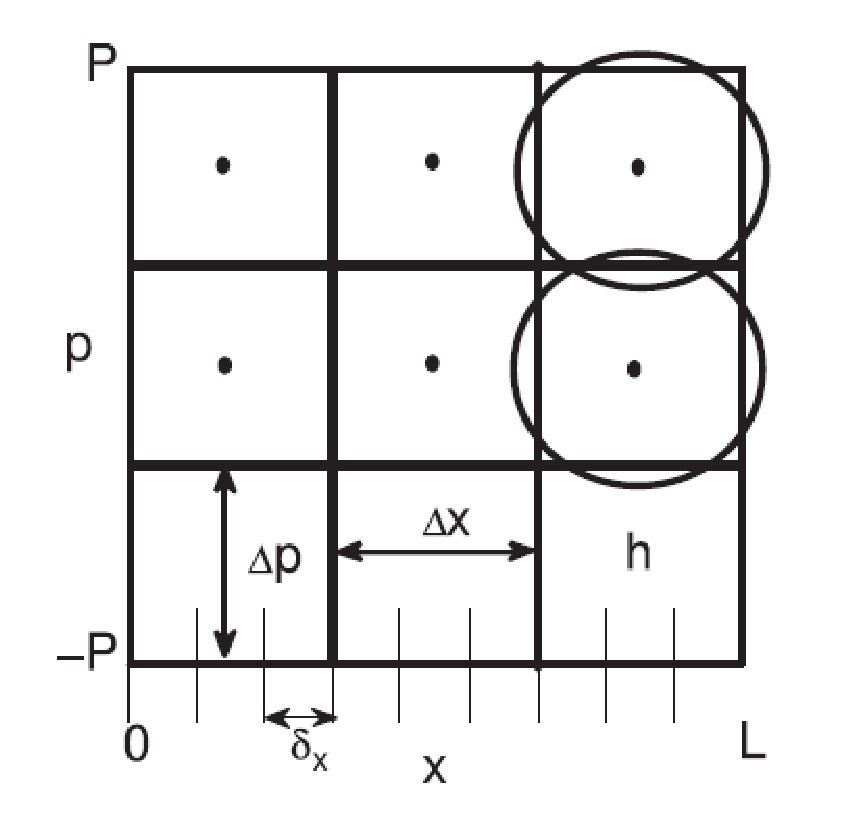
\includegraphics[scale=0.5]{shim.eps}
\caption[Pictorial of ST basis functions]{9 sinc and $3\time3$ Von Neumann basis functions. The sinc functions are centred on the dashed lines on the bottom while the Von Neumann basis functions are centred in the middle of the squares. Figure taken from \Refc{Shimshovitz2012}}
\label{fig.r4}
\end{center}
\end{figure}

 From this, the basis functions are taken to be
\begin{equation}\label{eq.psfg}
\tilde{g}_{i,j}\left(x\right)=\sum_{n=1}^{N}\phi_n\left(x_n\right)g_{i,j}\left(x_n\right).
\end{equation}
If a $G$ matrix is defined with elements $G_{k,l}=g_{l}\left(x_k\right)$, where $l$ runs over all $i,j$ values, than Eq.~(\ref{eq.psfg}) can be rewritten as $\tilde{G}=\Phi G$. Since $\int \phi_m\left(x\right)\phi_n\left(x\right)$ is diagonal, the matrix representation is
\begin{equation}\label{eq.psfg2}
H_{i,j,i^{\prime},j^{\prime}}U=
\sum_{m=1}^{N}\sum_{n=1}^{N}g_{i,j}\left(x_m\right)\left(\int \phi_m\left(x\right)H\phi_n\left(x\right)\right)g_{i^{\prime},j^{\prime}}\left(x_n\right)U=SU
\end{equation}
This basis turns out to not be conducive to pruning in that every basis function removed decreases the accuracy of the eigenvalues.  If you instead use basis functions $b_{k}\left((x\right)=\sum_{l=1}^N\tilde{g_{l}}\left(S^{-1}\right)_{l,k}$ then it results in the matrix representation
\begin{equation}\label{eq.psfg3}
H_{k,l}U=.\sum_{m=1}^{N}\sum_{n=1}^{N}b_{l}\left(x_m\right)\left(\int \phi_m\left(x\right)H\phi_n\left(x\right)\right)b_{k}\left(x_n\right)U=S^{-1}U
\end{equation}
which can be pruned without decreasing the accuracy.  
